\section{Aufbau}
Der Versuchsaufbau besteht im wesentlichen aus einem Justierlaser ($\lambda = 532\,\text{nm}$, $P_{Max}$ = 1 \, \text{mW}), einer Blende, einem Laserrohr mit Helium und Neon, eine Stromquelle
sowie zwei Resonatorspiegel mit Justierschrauben. 

\begin{figure}
  \centering
  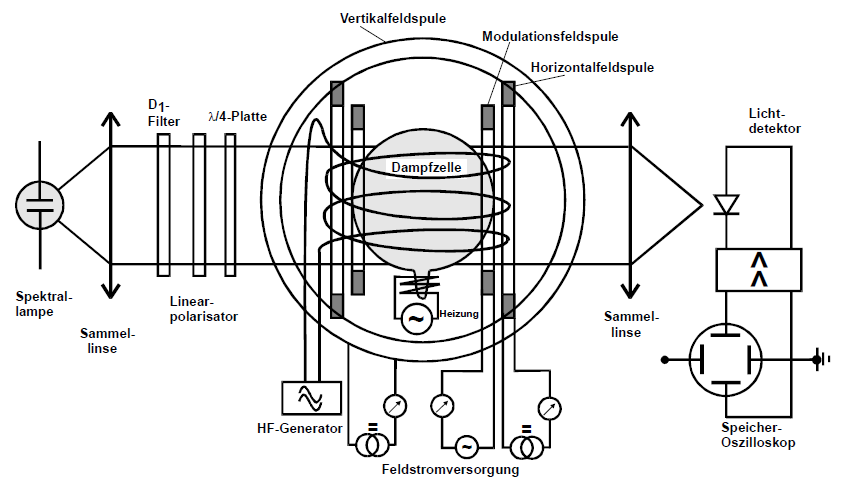
\includegraphics[width=0.75\textwidth]{img/aufbau.png}
  \caption{Energieniveaus im HeNe-Laser}
  \label{abb:aufbau}
\end{figure}

Alle optischen Elemente werden auf einer Justageschiene montiert und mit Hilfe des Justagelasers an die optische Achse angepasst.
Sobald alle optischen Elemente justiert wurden, wird die Stromquelle auf $I_{Max} = 6,5 \text{mA}$ gestellt. Nun wird im Lasermedium
eine Besetzungszahlinversion erzeugt, was sich in einem Leuchten in der Farbe des korrespondierenden Überganges zeigt. In der Regel,
reicht diese erste Justage nicht um den Aufbau zum "Lasern" zu bringen. Jedoch reicht oft eine Minimale nachjustage der Resonatorspiegel.
Am Ende der Justageschiene findet sich verschiedene messtechnische Komponenten wie Photodiode, Blenden, Mikrometerschraube etc. 
um das Licht untersuchen zu können.

\section{Durchführung}
Zu Beginn muss der Versuchsaufbau justiert werden. Nach der Justage wird die Stromquelle auf $I = 6,5 \, \text{mA}$ eingestellt.
Danach werden die Justageschrauben an den Resonatorspiegel leicht angepasst, sodass die Lasettätigkeit einsetzt. An dieser Stelle
kann damit begonnen werden die Stabilitätsbedingung zu überprüfen. Dafür wird zu begin der minimale Resonatorabstand eingestellt
und sukzessiv der Abstand erhöht und Nachjustiert. Dieses vorgehen wird so lange wiederholt bis der Resonator nicht mehr stabil
betrieben werden kann.

Anschliedend werden die TEM-Moden ausgemessen, wobei Ausschließlich die $LP_{00}$ und die $LP_{01}$ Mode betrachtet werden.
Die $LP_{00}$ Mode kann ohne weiteres mit Hilfe der Photodiode ausgemessen werden. Für die $LP_{02}$ muss voher eine Modenblende in den 
Resonator eingebracht werden. 

Abschließend wird die longitudinale Resonatormode mit Hilfe eines Frequenzanalysator auf die beteiligten Frequenzkomponenten untersucht.


